% Fleet Console: two-page project report (French). Compile with XeTeX: tectonic -X compile main_fr.tex
\documentclass[9pt,a4paper]{extarticle}
\usepackage[french]{babel}
% Visual style of the two-page report: Times-like serif (TeX Gyre Termes), near-black ink, no colour outside screenshots and icons.
% Compiled with XeTeX (tectonic).
\usepackage{fontspec}
\setmainfont{texgyretermes}[Extension=.otf, UprightFont=*-regular, BoldFont=*-bold, ItalicFont=*-italic, BoldItalicFont=*-bolditalic]% metric clone of Times New Roman
\setmonofont{texgyrecursor}[Extension=.otf, UprightFont=*-regular, BoldFont=*-bold, Scale=0.95]
\newcommand{\lightfont}{\mdseries}
\newcommand{\mediumfont}{\bfseries}

\usepackage[a4paper,margin=14mm]{geometry}
\usepackage{xcolor}
\usepackage{tikz}
\usetikzlibrary{arrows.meta,positioning,calc,fit,backgrounds}
\usepackage{graphicx}
\usepackage{enumitem}
\usepackage{array}
\usepackage{colortbl}
\usepackage{microtype}
\usepackage{etoolbox}
\usepackage{xstring}

\definecolor{ink}{HTML}{0A0B0D}
\definecolor{secondary}{RGB}{255,117,92}
\definecolor{hairline}{HTML}{0A0B0D}% rules and frames are black
\definecolor{grey}{HTML}{6B6E73}
\definecolor{wash}{HTML}{F3F4F5}
\color{ink}

\setlength{\parindent}{0pt}
\setlength{\parskip}{0pt}
\setlength{\columnsep}{6mm}
\pagestyle{empty}
\setlist{nosep, leftmargin=*, itemsep=0.8pt, topsep=0pt, label=\textcolor{ink}{\textbullet}}
\linespread{1.02}
\emergencystretch=2em

% Section title in sentence case; the optional argument adds space above it.
\newcommand{\rsection}[2][0mm]{%
  \par\vspace{\dimexpr 4.5mm+#1\relax}%
  {\fontsize{12}{14}\selectfont\mediumfont #2\par}%
  \vspace{1.5mm}}

% Screenshot with rounded corners; a named grey placeholder if the file is missing.
\newsavebox{\shotbox}
\newlength{\shotw}
\newlength{\shoth}
\newcommand{\shotratio}{0.52}
\newcommand{\shotzoom}{1}
\newcommand{\shotfocus}{0}
\newcommand{\shotfocusx}{0.5}% 0 shows the left edge, 0.5 the centre, 1 the right edge
\newcommand{\shot}[3]{%
  \setlength{\shotw}{#2}%
  \setlength{\shoth}{\shotratio\shotw}%
  \begin{minipage}[t]{\shotw}\centering
    \IfFileExists{images/#1}{%
      \sbox{\shotbox}{\includegraphics[width=\shotzoom\shotw]{images/#1}}%
      \ifdim\ht\shotbox<\shoth \sbox{\shotbox}{\includegraphics[height=\shoth]{images/#1}}\fi
      \begin{tikzpicture}[baseline=(current bounding box.north)]
        \useasboundingbox (0,0) rectangle (\shotw,\shoth);
        \clip[rounded corners=2mm] (0,0) rectangle (\shotw,\shoth);
        \node[anchor=north west, inner sep=0] at ({-\shotfocusx*(\wd\shotbox-\shotw)},{\shoth+\shotfocus*(\ht\shotbox-\shoth)}) {\usebox{\shotbox}};
      \end{tikzpicture}%
    }{%
      \begin{tikzpicture}[baseline=(current bounding box.north)]
        \fill[wash, rounded corners=2mm] (0,0) rectangle (\shotw,\shoth);
        \node[font=\fontsize{7}{8}\selectfont\ttfamily, text=secondary] at (0.5\shotw,0.5\shoth) {\detokenize{#1}};
      \end{tikzpicture}%
    }\\[0.8mm]
    {\fontsize{7}{8}\selectfont\color{secondary}#3}%
  \end{minipage}}

% Technical-choice table: domain and choice, reason, discarded alternative with the reason it was discarded.
% The first line of the table sits on the first baseline of the bullets next to it (both blocks are top-aligned).
\newenvironment{choixtable}{%
  \fontsize{8}{9.4}\selectfont
  \setlength{\tabcolsep}{2pt}%
  \begin{tabular*}{\linewidth}[t]{@{}>{\raggedright\arraybackslash}p{0.31\linewidth}@{\extracolsep{\fill}}>{\raggedright\arraybackslash}p{0.30\linewidth}>{\raggedright\arraybackslash}p{0.34\linewidth}@{}}%
  {\mediumfont Domaine et choix} & {\mediumfont Pourquoi} & {\mediumfont Alternative écartée}\\[0.2mm]
  \arrayrulecolor{ink}\hline\noalign{\vspace{0.4mm}}}{%
  \end{tabular*}}
\newcommand{\choix}[4]{\textbf{#1}\newline #2 & #3 & \textcolor{secondary}{#4}\\[0.2mm]\arrayrulecolor{hairline}\hline\noalign{\vspace{0.4mm}}}

% Difficulty block: a short labelled paragraph behind a thin left rule.
\newcommand{\difficulte}[3]{%
  \par\vspace{2.5mm}\noindent%
  \begin{tikzpicture}[baseline=(box.north)]
    \node[inner sep=0, text width=\dimexpr\linewidth-3mm\relax, align=justify, anchor=north west] (box) at (3mm,0) {%
      \fontsize{8.5}{10.2}\selectfont
      {\fontsize{8.5}{10.2}\selectfont\mediumfont Difficulté :}\hspace{1.5mm}#2\par\vspace{0.5mm}#3};
    \draw[hairline, line width=0.8pt] ([xshift=-1.5mm]box.north west) -- ([xshift=-1.5mm]box.south west);
  \end{tikzpicture}\par}


% Shared TikZ styles for the report figures: line styles stand for flow types, no colour.
\definecolor{lightgrey}{HTML}{B9BBBF}
\tikzset{
  lab/.style={font=\fontsize{7}{8}\selectfont, text=ink, align=center, inner sep=1pt},
  sub/.style={font=\fontsize{6}{7}\selectfont, text=secondary, align=center, inner sep=1pt},
  flowT/.style={-{Stealth[length=1.7mm,width=1.3mm]}, line width=0.6pt, draw=ink},
  flowC/.style={-{Stealth[length=1.7mm,width=1.3mm]}, line width=0.6pt, draw=ink, dash pattern=on 3pt off 2pt},
  flowV/.style={line width=0.8pt, draw=ink, dash pattern=on 0.2pt off 2.2pt, line cap=round},
  flowD/.style={-{Stealth[length=1.7mm,width=1.3mm]}, line width=0.6pt, draw=lightgrey},
  flowJ/.style={-{Stealth[length=1.5mm,width=1.1mm]}, line width=0.4pt, draw=ink},
  lane/.style={draw=hairline, line width=0.4pt, rounded corners=2mm},
}
\providecommand{\mk}[1]{node[circle, fill=ink, text=white, inner sep=0.7pt, minimum size=3.1mm, font=\fontsize{6}{6}\selectfont\bfseries, midway]{#1}}
\providecommand{\ico}[4]{%
  \node[inner sep=0] (#1) at (#2) {\includegraphics[height=7mm]{icons/#3.pdf}};
  \node[lab, below=0pt of #1] (#1l) {#4};}
\providecommand{\icoa}[4]{%
  \node[inner sep=0] (#1) at (#2) {\includegraphics[height=7mm]{icons/#3.pdf}};
  \node[lab, above=0pt of #1] (#1l) {#4};}
\providecommand{\icow}[4]{%
  \node[inner sep=0] (#1) at (#2) {\includegraphics[height=7mm]{icons/#3.pdf}};
  \node[lab, left=1pt of #1] (#1l) {#4};}

\usepackage[hidelinks]{hyperref}


\begin{document}
\sloppy

% ---------- Header ----------
\noindent{\fontsize{22}{24}\selectfont\mediumfont Interface de contrôle d'une flotte de robots}\\[1mm]
{\fontsize{10}{12}\selectfont\itshape Superviser, téléopérer et mesurer une flotte de robots logistiques déjà déployée}\\[1.6mm]
{\fontsize{7.5}{9}\selectfont Vincent Lucas ·
\href{https://www.linkedin.com/in/vincent-lucas-483b29295/}{\underline{LinkedIn}} ·
\href{https://github.com/vinsl/robot-fleet-console}{\underline{Code source}}\\
\color{secondary}Projet personnel effectué du 30 octobre au 5 novembre 2026}

% ---------- Contexte ----------
\rsection{Contexte}
\noindent\begin{minipage}[t]{0.50\linewidth}\vspace{0pt}
  \fontsize{8.7}{10.3}\selectfont
  Une flotte de robots logistiques autonomes travaille déjà chez des clients, mais aucun outil ne la rend encore visible et pilotable à distance. Ce projet propose une réponse complète, de l'infrastructure à l'interface, déployée sur AWS et testée de bout en bout. Le viewer, par exemple le responsable du site client, suit la flotte en lecture seule. L'opérateur reçoit les alertes et prend la main sur un robot depuis son téléphone ou son ordinateur.\par\vspace{1mm}
  La CI/CD et les contrôles de sécurité ont précédé le code produit. J'ai ensuite conçu l'infrastructure, designé le code et piloté des agents IA spécialisés en code, tests et revue de sécurité. Chaque décision est consignée dans l'un des 69 ADR, et chaque PR passe la CI et une revue avant fusion.
\end{minipage}\hfill
\begin{minipage}[t]{0.47\linewidth}\vspace{0pt}
  \renewcommand{\shotzoom}{1}\renewcommand{\shotratio}{0.464}\shot{fleet-view.png}{\linewidth}{Vue flotte en direct, 9 robots en ligne}
\end{minipage}

% ---------- Périmètre ----------
\rsection{Périmètre du projet}
\noindent\begin{minipage}[t]{0.485\linewidth}\vspace{0pt}
  \fontsize{8.5}{10.3}\selectfont
  {\mediumfont Inclus}\par\vspace{0.6mm}
  \begin{itemize}
    \item Proposer une architecture cloud sécurisée, déployée à partir du code.
    \item Superviser une flotte et la téléopérer en sécurité, avec verrou, deadman et arrêt d'urgence.
    \item Garder la trace de chaque alerte, commande et prise de contrôle pour l'audit et les KPI.
  \end{itemize}
\end{minipage}\hfill
\begin{minipage}[t]{0.485\linewidth}\vspace{0pt}
  \fontsize{8.5}{10.3}\selectfont
  {\mediumfont Exclus}\par\vspace{0.6mm}
  \begin{itemize}
    \item Déplacer de vrais robots : l'agent réel tourne sur une VM et le reste de la flotte est simulé.
    \item Prendre le contrôle d'un vrai robot : les pannes sont simulées et la console donne accès à leur résolution. Il resterait à relier l'agent au robot.
    \item Pousser la simulation : elle sert seulement à valider l'interface.
  \end{itemize}
\end{minipage}

% ---------- Infrastructure ----------
\rsection{Infrastructure}
\noindent% Architecture diagram: robots | AWS eu-west-3 | users, with a deployment band underneath.
% The console is a web application served by the platform, distinct from the people who use it.
% Line style carries the flow type (solid telemetry, dashed commands, dotted video, grey deployment).
% Coordinates are in centimetres; the picture is 18.2 cm wide, the text width.
\begin{tikzpicture}[x=1cm,y=1cm]
  % Lanes.
  \draw[lane] (0,2.2) rectangle (2.9,5.95);
  \node[sub, anchor=north west] at (0.12,5.9) {Robots};
  \draw[lane, fill=wash!60] (3.5,0.1) rectangle (14.6,6.3);
  \node[sub, anchor=north west] at (3.65,6.22) {AWS · eu-west-3};
  \draw[lane] (15.9,0.9) rectangle (18.2,5.95);
  \node[sub, anchor=north west] at (16.02,5.9) {Utilisateurs};

  % Robot lane.
  \ico{cam}{1.45,5.1}{Res_IoT_Thing_Camera}{Caméra}
  \ico{agent}{1.45,3.5}{Res_IoT_Thing_Generic}{Agent Python}
  \node[sub, below=0pt of agentl] {X.509 · deadman local};

  % AWS components.
  \icoa{iot}{4.9,3.5}{AWS-IoT-Core}{IoT Core}
  \ico{sqs}{7.1,3.5}{Amazon-Simple-Queue-Service}{SQS}
  \draw[rounded corners=1.5mm, fill=white, draw=hairline, line width=0.4pt] (8.3,2.85) rectangle (11.7,4.15);
  \node[inner sep=0] (lam) at (8.85,3.5) {
\includegraphics[height=7mm]{icons/AWS-Lambda.pdf}};
  \node[sub, anchor=west, align=left, text=ink] at (9.25,3.5)
    {ingest · control · alerts\\audit · kpi · site · ws};
  \icoa{ddb}{10,5.1}{Amazon-DynamoDB}{DynamoDB}
  \ico{ws}{13.4,3.5}{Amazon-API-Gateway}{API Gateway\\WebSocket}
  \ico{http}{10.9,1.5}{Amazon-API-Gateway}{API Gateway HTTP}
  \ico{cog}{13.4,1.5}{Amazon-Cognito}{Cognito}
  \ico{kvs}{4.9,5.1}{Amazon-Kinesis-Video-Streams}{KVS (signalisation)}
  % Console web: one entity (S3 origin behind CloudFront), grouped in a light box facing the users.
  \draw[rounded corners=1.5mm, fill=white, draw=hairline, line width=0.4pt] (11.4,4.4) rectangle (14.4,6.15);
  \node[lab] at (12.9,5.9) {Console web (React)};
  \node[inner sep=0] (s3) at (12.3,5.15) {
\includegraphics[height=7mm]{icons/Amazon-Simple-Storage-Service.pdf}};
  \node[inner sep=0] (cf) at (13.5,5.15) {
\includegraphics[height=7mm]{icons/Amazon-CloudFront.pdf}};
  \node[sub] at (12.9,4.6) {hébergée sur S3 + CloudFront};
  \ico{cw}{5.4,1.3}{Amazon-CloudWatch}{CloudWatch}
  \ico{sns}{7.2,1.3}{Amazon-Simple-Notification-Service}{SNS alarmes}

  % Users lane: people on their own phone or computer, signed in with Cognito.
  \node[inner sep=0] (usr) at (17.05,4.75) {
\includegraphics[height=7mm]{icons/Res_Users.pdf}};
  \node[inner sep=0] (mob) at (16.55,3.65) {
\includegraphics[height=7mm]{icons/Res_Mobile-client.pdf}};
  \node[inner sep=0] (pc) at (17.55,3.65) {
\includegraphics[height=7mm]{icons/Res_Client.pdf}};
  \node[lab, anchor=north] (usrl) at (17.05,3.05) {Opérateur · Viewer};
  \node[sub, below=0pt of usrl] {téléphone ou\\ordinateur personnel};

  % Telemetry (solid): robot to IoT Core, rule to SQS, batch to Lambda, then database and push.
  \draw[flowT] ([yshift=1.2mm]agent.east) -- ([yshift=1.2mm]iot.west) \mk{1};
  \draw[flowT] (iot.east) -- node[above, sub]{règle IoT} (sqs.west);
  \draw[flowT] (sqs.east) -- (8.3,3.5);
  \draw[flowT] (10,4.15) -- (ddb.south);
  \draw[flowT] (11.7,3.5) -- (ws.west);
  \draw[flowT] (ws.east) -- (15.9,3.5);

  % Commands and acknowledgements (dashed): browser to HTTP API, control Lambda to IoT Core, back to the robot.
  \draw[flowC] (17.05,0.9) -- (17.05,0.5) -- (10.9,0.5) \mk{2} -- (10.9,0.62);
  \draw[flowC] (10.9,2.2) -- (10.9,2.85);
  \draw[flowC] (8.7,2.85) -- (8.7,2.35) -- (4.9,2.35) -- (iot.south);
  \draw[flowC] ([yshift=-1.2mm]iot.west) -- ([yshift=-1.2mm]agent.east);
  \draw[flowJ] (cog.west) -- node[above, sub]{jeton d'accès} (http.east);
  \draw[flowJ, {Stealth[length=1.5mm,width=1.1mm]}-{Stealth[length=1.5mm,width=1.1mm]}] (15.9,1.5) -- (cog.east);
  \node[sub] at (15.25,1.88) {identifiants\\+ TOTP};
  \draw[flowJ] (cf.east) -- (15.9,5.15);
  \node[sub] at (15.25,5.53) {charge\\l'application};

  % Video (dotted): peer to peer, KVS only carries the signalling.
  \draw[flowV] (cam.north) -- (1.45,6.75) -- (17.05,6.75) -- (17.05,5.95);
  \path (6,6.75) -- (14,6.75) \mk{3};
  \draw[flowV] (kvs.north) -- (4.9,6.75);

  % Alarms.
  \draw[flowJ] (cw.east) -- (sns.west);

  % Deployment (light grey): CI to Terraform to AWS.
  \node[lab, anchor=east] at (3.4,-0.75) {Déploiement};
  \node[inner sep=0] (gh) at (3.9,-0.75) {
\includegraphics[height=5.5mm]{icons/Res_Git-Repository.pdf}};
  \node[lab, anchor=west] (ghl) at (4.2,-0.75) {GitHub Actions};
  \node[lab, draw=hairline, rounded corners=1mm, inner sep=2.5pt] (oidc) at (8.4,-0.75) {OIDC · aucune clé longue durée};
  \node[lab, draw=hairline, rounded corners=1mm, inner sep=2.5pt] (tf) at (12.2,-0.75) {Terraform · plan relu en PR};
  \draw[flowD] (ghl.east) -- (oidc.west);
  \draw[flowD] (oidc.east) -- (tf.west);
  \draw[flowD] (tf.east) -- (14.3,-0.75) -- (14.3,0.1);
  \node[sub, anchor=west, align=left] at (14.45,-0.4) {déploie l'infra et\\publie la console};
  \path (ghl.east) -- (oidc.west) \mk{4};
  % Line-style legend in the free corner under the robots lane.
  \foreach \y/\st/\txt in {1.95/flowT/télémétrie, 1.6/flowC/commandes, 1.25/flowV/vidéo, 0.9/flowJ/authentification et console, 0.55/flowD/déploiement}{
    \draw[\st] (0.1,\y) -- (0.75,\y);
    \node[sub, anchor=west, align=left] at (0.85,\y) {\txt};
  }
\end{tikzpicture}
\par\vspace{0.3mm}
{\fontsize{7.5}{9}\selectfont\color{grey}
\textbf{\color{ink}1} télémétrie de 0,5 à 2 Hz, lots de 100 ou 1 s \quad
\textbf{\color{ink}2} commande, cible p95 < 500 ms \quad
\textbf{\color{ink}3} vidéo WebRTC peer to peer \quad
\textbf{\color{ink}4} 8 min du merge à la production}
\par\vspace{0.8mm}

\noindent\begin{minipage}[t]{0.485\linewidth}\vspace{0pt}
  \fontsize{8.5}{10.3}\selectfont
  \begin{itemize}
    \item AWS fournit des briques éprouvées pour une flotte, comme IoT Core et l'identité X.509 de chaque robot. Le protocole entre robots et cloud est versionné et validé aux deux bouts, et la logique métier est testée sans AWS.
    \item Tout est décrit en Terraform. Un merge atteint la production en 8 minutes, et un robot ou un site s'ajoute sans toucher au code.
    \item Pour 20 robots actifs 12 h par jour, l'estimation est de 65~\$ par mois, soit 3~\$ par robot. Au repos, la plateforme coûte moins de 5~\$ par mois, et tout le développement a coûté 0,16~\$.
    \item Les mesures arrivent par lots et les positions vont droit aux écrans par WebSocket. DynamoDB garde l'état, les alertes 90 jours et l'audit un an, et 37 alarmes surveillent les erreurs.
  \end{itemize}
\end{minipage}\hfill
\begin{minipage}[t]{0.485\linewidth}\vspace{0pt}
  \begin{choixtable}
    \choix{Langages}{TypeScript, Python}{types partagés, Python côté robot}{tout en TypeScript, loin de la robotique}
    \choix{Back end}{fonctions Lambda}{aucun serveur, coût à l'usage}{Fargate, facturé sans trafic}
    \choix{Robots}{IoT Core, MQTT}{identité X.509 par robot}{broker auto-hébergé à sécuriser soi-même}
    \choix{Données}{DynamoDB}{accès par clé, à la demande}{Aurora Serverless, coût plancher}
    \choix{Déploiement}{AWS, Terraform}{plan relu en PR, rejouable}{CDK, lié à CloudFormation}
  \end{choixtable}
\end{minipage}

\difficulte{}{La CI ne pouvait pas s'authentifier auprès d'AWS}{Le job de plan Terraform échouait 12 fois de suite. GitHub signe ses jetons OIDC avec les identifiants numériques du dépôt, alors que la confiance IAM attendait son nom. Réécrite sur l'identifiant immuable et sans joker, elle passe. Je vérifie désormais le réglage réel avant la documentation.}

\newpage
% ---------- Sécurité ----------
\rsection{Sécurité}
\noindent\begin{minipage}[c]{0.70\linewidth}
  % Safety strip, narrowed so that the OWASP ZAP table can sit to its right.
% Both paths go through the control Lambda; the E-STOP one skips the lock check (ADR 0062).
\begin{tikzpicture}[x=0.62cm,y=1cm]
  \ico{op}{1.0,0.55}{Res_Users}{Opérateur}
  \ico{ctl}{6.2,0.55}{AWS-Lambda}{control}
  \node[sub, below=0pt of ctll] {garde le jeton de verrou};
  \ico{iot}{11.4,0.55}{AWS-IoT-Core}{IoT Core}
  \ico{rob}{16.6,0.55}{Res_IoT_Thing_Generic}{Robot}
  \node[sub, below=0pt of robl] {deadman 1 s → PAUSED};
  \draw[flowC] (op.east) -- node[above, sub]{commande · verrou requis} (ctl.west);
  \draw[flowC] (ctl.east) -- (iot.west);
  \draw[flowC] (iot.east) -- (rob.west);
  \draw[flowC, line width=1pt] (op.north) -- (1.0,1.45) -- node[above, lab, fill=white, inner sep=1.5pt]{\bfseries E-STOP · prioritaire, sans verrou\\\mdseries verrouillé jusqu'à libération} (6.2,1.45) -- (ctl.north);
\end{tikzpicture}

\end{minipage}\hfill
\begin{minipage}[c]{0.28\linewidth}\raggedleft
  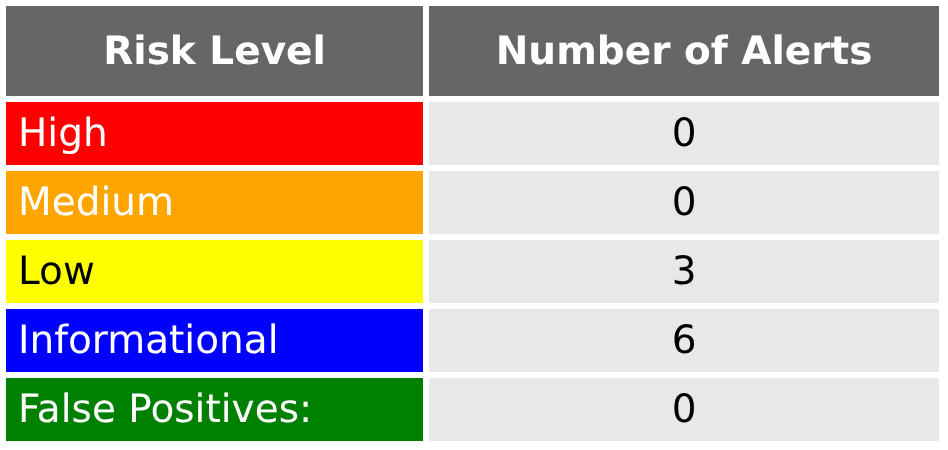
\includegraphics[width=0.95\linewidth]{images/zap-summary.png}\\[0.6mm]
  {\fontsize{6.5}{7.8}\selectfont\color{secondary}OWASP ZAP 2.17, scan baseline, 4 novembre 2026}
\end{minipage}\par\vspace{2mm}
\noindent\begin{minipage}[t]{0.485\linewidth}\vspace{0pt}
  \fontsize{8.5}{10.3}\selectfont
  \begin{itemize}
    \item Les comptes sont créés par un administrateur et chaque rôle passe par un TOTP. Aucune clé AWS longue durée n'existe : SSO pour les humains, OIDC pour la CI, X.509 pour les robots.
    \item Chaque Lambda a son propre rôle IAM, et un robot ne publie que sur ses propres topics, ce qui a été vérifié en réel.
    \item Un seul opérateur pilote un robot et son verrou expire après 30 s d'inactivité. Le deadman du robot le met en pause après 1 s sans battement, même réseau coupé.
    \item L'arrêt d'urgence passe avant tout, mais reste logiciel et complète une sécurité matérielle. Le modèle STRIDE recense 71 menaces, et au moins 51 tests vérifient des accès refusés.
  \end{itemize}
\end{minipage}\hfill
\begin{minipage}[t]{0.485\linewidth}\vspace{0pt}
  \begin{choixtable}
    \choix{Utilisateurs}{Cognito, MFA TOTP}{non contournable}{MFA géré par l'application, contournable par oubli}
    \choix{Robots}{X.509, politique IoT}{un seul document à auditer}{une politique par robot}
    \choix{Contrôle}{verrou dans le cloud}{invisible au navigateur}{jeton côté client, exposé à un script}
    \choix{Règles}{machine d'états partagée}{mêmes règles cloud et robot}{deux implémentations qui divergent}
    \choix{Réseau}{pas de VPC}{sécurité par l'identité}{VPC avec NAT, 30 € par mois sans gain}
  \end{choixtable}
\end{minipage}

\difficulte{}{Un arrêt d'urgence pouvait rester sans accusé}{En coupure réseau, la file d'envoi du robot, limitée à 100 messages, pouvait se remplir et refuser l'accusé d'un arrêt d'urgence. Huit places sont désormais réservées aux messages d'arrêt, avec un test qui remplit la file. Une limite qui écarte des messages doit toujours laisser passer l'arrêt.}

% ---------- Aperçu et interface ----------
\rsection[5mm]{Aperçu et interface}
\renewcommand{\shotzoom}{1}\renewcommand{\shotratio}{0.457}\noindent\shot{robot-page-video.png}{0.47\linewidth}{Page robot : vidéo en direct, latence de 42 ms}\hfill
\renewcommand{\shotratio}{0.82}\renewcommand{\shotzoom}{1.8}\renewcommand{\shotfocusx}{0}\shot{14-open-major-alert.png}{0.255\linewidth}{Alerte majeure ouverte}\hfill
\renewcommand{\shotzoom}{1}\shot{18-audit-log.png}{0.255\linewidth}{Journal d'audit filtrable}\par\vspace{1.5mm}
\noindent\begin{minipage}[t]{0.485\linewidth}\vspace{0pt}
  \fontsize{8.5}{10.3}\selectfont
  \begin{itemize}
    \item Le plan du site occupe l'écran. Au repos, seuls la ligne d'état, deux KPI et le dock restent visibles.
    \item Les pictogrammes et le design ont été validés en amont du code. On compte 9 états de robot et 8 badges qui précisent l'information, pour représenter 28 situations différentes.
    \item Une alerte mène au robot concerné et la pause part en 3 clics.
    \item Un état se lit par sa forme, son icône et son texte, jamais par la couleur seule. WCAG AA, clavier, français, anglais, téléphone.
  \end{itemize}
\end{minipage}\hfill
\begin{minipage}[t]{0.485\linewidth}\vspace{0pt}
  \begin{choixtable}
    \choix{Front end}{React, TypeScript, Vite}{statique, coût nul au repos}{Next.js, un serveur sans besoin}
    \choix{État}{Zustand, TanStack Query}{temps réel séparé du serveur}{Redux, plus de code}
    \choix{Styles}{CSS Modules, tokens}{compatible avec la CSP}{CSS-in-JS, refusé par la CSP}
    \choix{Tests}{Vitest, Playwright}{scénario rejoué en déployé}{mocks seuls, aveugles au déploiement}
  \end{choixtable}
\end{minipage}

\difficulte{}{Trouver le bon niveau de simulation}{Valider l'interface demandait une flotte simulée assez crédible, mais la limite de ce qui suffisait était difficile à fixer. J'ai passé beaucoup de temps sur des trajets A*, la réservation des postes de travail et l'évitement entre robots, alors que la simulation ne faisait pas partie des objectifs. Depuis, je compare chaque ajout aux objectifs du projet et je range le reste dans une liste de bonus classés, pour que le MVP soit prêt à temps. Savoir recentrer un projet sur l'essentiel fait partie du travail.}

% ---------- Recul ----------
\rsection[5mm]{Recul}
\noindent\begin{minipage}[t]{0.485\linewidth}\vspace{0pt}
  \fontsize{8.5}{10.3}\selectfont
  {\mediumfont Ce que je ferais autrement}\par\vspace{0.6mm}
  \begin{itemize}
    \item Tester sur l'environnement déployé dès le premier jour, car le test réel a apporté la plupart des correctifs d'interface.
    \item Utiliser une caméra d'au moins 15 images/s. Celle de la VM en donnait 1 à 3, trop peu pour mesurer la latence vidéo.
  \end{itemize}
\end{minipage}\hfill
\begin{minipage}[t]{0.485\linewidth}\vspace{0pt}
  \fontsize{8.5}{10.3}\selectfont
  {\mediumfont Ce qui manque avant la production}\par\vspace{0.6mm}
  \begin{itemize}
    \item Un robot réel en mouvement via ROS 2, derrière une sécurité matérielle.
    \item La résolution automatique des alertes et un Data Lake pour l'analyse.
    \item Le multi-site isolé par client, déjà prévu dans les clés de données, et un WAF.
    \item Des lots de 5 mesures par message MQTT, soit 35 \% de coût en moins pour 5 s de fraîcheur.
  \end{itemize}
\end{minipage}
\end{document}
